\section{Results and Figures}\label{sec:figures}
%%%%%%%%%%%%%%%%%%%%%%%%%%%%%%%%%%%%%%%%%%%%%%%%%%%%%%%%%%%%%%%%%%%%
\subsection{Part I - Mathematical modelling}\label{subsec:part1}
\subsubsection{Problem 1}

In the following derivations, Newton's 2nd law of motion for rotation is used:

\begin{equation}\label{eq:P1_N2}
    J \dot{\omega} = \sum \tau
\end{equation}
Computing the equations of motion around the pitch using~\cref{eq:P1_N2},~\cref{fig:heli} and \cref{eq:P1_forces_propellers}:
\begin{align}
    J_p \ddot{p} &= l_p F_f - l_p F_b \nonumber \\
    J_p \ddot{p} &= l_p K_f V_f - l_p K_f V_b \nonumber \\
    J_p \ddot{p} &= l_p K_f (V_f - V_b) \nonumber \\
    J_p \ddot{p} &= L_1 V_d, \quad L_1 = l_p K_f \quad V_d = V_f - V_b
    \label{eq:P1_pitch_non-linear}
\end{align}
For the elevation we also use the same procedure
\begin{align}
    J \dot{\omega} &= \sum \tau \nonumber \\
    J_e \ddot{e} &= g l_c m_c \cos{e} - 2 g l_h m_p \cos{e} + K_f l_h V_f \cos{p} + K_f l_h V_b \cos{p} \nonumber \\
    J_e \ddot{e} &= L_2 \cos{e} + L_3 V_s \cos{p}, \label{eq:P1_elevation_non-linear}\\    
                 &  \quad L_2 = g (l_c m_c - 2 l_h m_p),
                    \quad L_3 = K_f l_h,
                    \quad V_s = V_f + V_b \nonumber
\end{align}
Finally we need to calculate the travel
\begin{align}
    J \dot{\omega} &= \sum \tau \nonumber \\
    J\ddot{\lambda} &= -(K_f l_h V_f + K_f l_h V_b)\cos{e}\sin{p} \nonumber \\
    J\ddot{\lambda} &= L_4 V_s \cos{e} \sin{p},
                        \quad L_4 = - K_f l_h
                        \label{eq:P1_travel_non-linear}
\end{align}
The reason for the negative sign is because a positive pitch gives a negative travel rate. The angles are because zero pitch angle gives zero travel rate, and zero elevation angle gives maximum travel rate.

To summarise we get the following constants
\begin{subequations}\label{eq:P1_constants_for_non-linear_eq}
    \begin{align}
        L_1 &= K_f l_p \label{eq:P1_L1} \\
        L_2 &= g (l_c m_c - 2 l_h m_p) \label{eq:P1_L2} \\
        L_3 &= K_f l_h \label{eq:P1_L3} \\
        L_4 &= -K_f l_h \label{eq:P1_L4}
    \end{align}
\end{subequations}

\subsubsection{Problem 2}
In this part we wish to linearise around the point
\begin{equation*}
    \begin{bmatrix}
        p \\
        e \\
        \lambda \\
    \end{bmatrix}
    =
    \begin{bmatrix}
        p^* \\
        e^* \\
        \lambda^* \\
    \end{bmatrix}
    =
    \begin{bmatrix}
        0 \\
        0 \\
        0 \\
    \end{bmatrix}
\end{equation*}
The linearisation will be with the helicopter horizontal in both pitch and elevation. As well as no travel. For the equilibrium point $V_d^*$ and $V_s^*$ needs to be determined. It's quite easy to imagine that $V_d^*$ will be zero, as anything else would give a $\dot{p} \neq 0$.

To derive $V_s^*$ it is possible to use the equations from last problem. Specifically \ref{eq:P1_elevation_non-linear}
\begin{align*}
     J_e \ddot{e} &= L_2 \cos{e} + L_3 V_s \cos{p} \\
     J_e * 0 &= L_2 + L_3 * V_s^* \\
     V_s^* &= -\frac{L2}{L3} \\
     V_s^* &= -\frac{g(l_c m_c - 2 l_h m_p)}{K_f l_h}
\end{align*}
To summarise
\begin{subequations}
    \begin{align}
        V_s^* &= -\frac{g(l_c m_c - 2 l_h m_p)}{K_f l_h} \label{eq:P1p2_Vs} \\
        V_d^* &= 0 \label{eq:P1p2_Vd}
    \end{align}    
\end{subequations}
To simplify further analysis, the following coordinate transformation is introduced.
\begin{equation}
    \begin{bmatrix}
        \tilde{p} \\ \tilde{e} \\ \tilde{\lambda}
    \end{bmatrix}
    =
    \begin{bmatrix}
        p \\ e \\ \lambda
    \end{bmatrix}
    -
    \begin{bmatrix}
        p^* \\ e^* \\ \lambda^*
    \end{bmatrix}
    \quad \text{and} \quad
    \begin{bmatrix}
        \tilde{V}_s \\ \tilde{V}_d
    \end{bmatrix}
    =
    \begin{bmatrix}
        V_s \\ V_d
    \end{bmatrix}
    -
    \begin{bmatrix}
        V_s^* \\ V_d^*
    \end{bmatrix}
\end{equation}
Which gives the following motion equations.
\begin{equation}
    \begin{bmatrix}
        p \\ e \\ \lambda
    \end{bmatrix}
    =
    \begin{bmatrix}
        \tilde{p} \\ \tilde{e} \\ \tilde{\lambda}
    \end{bmatrix}
    \quad \text{and} \quad
    \begin{bmatrix}
        V_s \\ V_d
    \end{bmatrix}
    =
    \begin{bmatrix}
        \tilde{V}_s \\ \tilde{V}_d
    \end{bmatrix}
    +
    \begin{bmatrix}
        -\frac{L_2}{L_3} \\ 0
    \end{bmatrix}
\end{equation}
To linearise we use the Jacobian and evaluate in our equilibrium
\begin{equation}
    a_{i,j} = \frac{\del f_i}{\del x_j}
\end{equation}

%%%%%%%%%%%%%%%%%%%%%%%%%%%%%%%%%%%%%%%%%%%%%%%%%%%%%%%%%%%%%%%%%%%%
\subsection{Part II - Monovariable Control}\label{subsec:part2}
Part II takes a look at PD and P controllers. The PD is for pitch, and P for travel rate. The following formulas describe the controllers.

\begin{align}
        \tilde{V}_d &= K_{pp} (\tilde{p}_c - \tilde{p}) - K_{pd}\td{p}  \label{eq:P2_PD}\\  
        \tilde{p}_c &= K_{rp} (\td{\lambda}_c - \td{\lambda}) \label{eq:P2_P}
\end{align}

\subsubsection{Problem 1}
It is possible to derive the dynamics of \eqref{eq:P2_PD} by replacing $\tilde{V}_d$ with the linearised equation from part I, \eqref{eq:P1_lin_eq_of_motion_p}.
\begin{align*}
    \tilde{V}_d &= K_{pp} (\tilde{p}_c - \tilde{p}) - K_{pd}\td{p}) \\
    \frac{\tdd{p}}{K_1} &= K_{pp} (\tilde{p}_c - \tilde{p}) - K_{pd}\td{p}) \\
    \tdd{p} &= K_1(K_{pp}(\tilde{p}_c - \tilde{p}) - K_{pd} \td{p})
\end{align*}
If we assume initial conditions to be zero, we arrive at the following laplace transform
\begin{align}
    s^2\tilde{P} &= K_1(K_{pp}(\tilde{P}_c - \tilde{P}) - sK_{pd} \tilde{P}  \nonumber \\
    \tilde{P} &= \frac{K_1 K_{pp}}{s^2 + K_1 K_{pd} s + K_1 K_{pp}} \tilde{P}_c \nonumber \\
    H(s) &= \frac{K_1 K_{pp}}{s^2 + K_1 K_{pd} s + K_1 K_{pp}}
\end{align}
From this, the following damping ratio and natural frequency follows
\begin{align}
    \zeta &= \frac{K_1 K_{pd}}{2\sqrt{K_1 K_{pp}}} \label{eq:P2_damping_ratio} \\
    \omega_0 &= \sqrt{K_1 K_{pp}} \label{eq:P2_natural_frequency}
\end{align}
This is familiar ground. For optimal behaviour, we choose $\zeta = 1$ as this corresponds to what is known as critical damping. Which in turn means the optimal damping, where the system is neither under or over damped.\\
With $\zeta = 1$, \eqref{eq:P2_damping_ratio} and \eqref{eq:P2_natural_frequency} yields 
\begin{align}
    K_{pd} = 2\sqrt{\frac{K_{pp}}{K_1}} \label{eq:P2_Kpd} \\
    K_{pp} = \frac{\omega_0^2}{K_1}. \label{eq:P2_Kpp} 
\end{align}
Finding an optimal $\omega_0$ is difficult, but as we can see in \eqref{eq:P2_Kpd}, $K_{pd}$ is purely dependent on $K_{pp}$ and the constant $K_1$. Thus, we can tune the pitch controller simply by testing different values of $K_{pp}$.\\
\\
To systematically test different values of $K_{pp}$, we created a simple matlab script that takes the pitch from $45\degree$ to $0\degree$ and tracks the response. Using a step \textit{down} to $0\degree$ like this is a good idea since our model is linearized around that value. We test for $K_{pp}$s ranging from $4$ to $20$ all the while holding the helicopter still at 0 elevation to isolate the pitch behaviour. Our findings, shown in Figure \ref{fig:P2p1_K_pp}, show that a $K_{pp}$ of about $10$ gives a rapid response without overshoot. With the 
\begin{itemize}
    \item $K_{pp} = 10$
    \item $K_{pd} = 6.65$
\end{itemize}
\begin{figure}[!!ht!!!!!!!!tb!!]
	\centering
		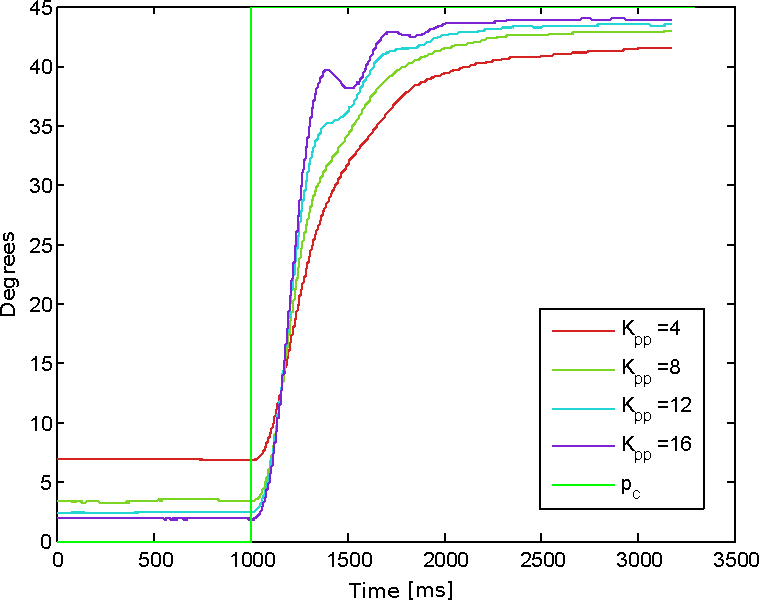
\includegraphics[width=1\textwidth,trim={0cm 0cm 0cm 0cm},clip]{figures/P2p1_K_pp_label.pdf}
	\caption{Pitch response with PD control}
\label{fig:P2p1_K_pp}
\end{figure}

\clearpage

\subsubsection{Problem 2}
The transfer function for the travel controller in \eqref{eq:P2_P} can be written as
\begin{equation}
    \frac{\td{\lambda}(s)}{\td{\lambda}_c(s)} = \frac{\rho}{s + \rho}, 
    \label{eq:P2_p_trasfer}
\end{equation}
where $\rho$ is a constant. To show this, we assume $\tilde p = \tilde p_c$ and get from \eqref{eq:P1_lin_eq_of_motion_l} that
\begin{align}
    \tilde{p} &= \frac{\tdd{\lambda}}{K_3} \label{eq:P2_p_to_lambda}.
\end{align}
Inserting this into \eqref{eq:P2_P} then yields
\begin{align*}
    \tdd{\lambda} &= K_3 K_{rp} (\td{\lambda}_c - \td{\lambda}),
\end{align*}
which in the laplace domain is
\begin{align*}
    s\td{\lambda} &= K_3 K_{rp} (\td{\lambda}_c - \td{\lambda}).
\end{align*}
Finally, by rearranging the terms, we get the transfer function 
\begin{align}
    h(s) = \frac{\td{\lambda}}{\td{\lambda}_c} = \frac{K_3 K_{rp}}{s + K_3 K_{rp}},
\end{align}
which when letting $\rho = K_3 K_{rp}$ becomes \eqref{eq:P2_p_trasfer}.
\begin{figure}[!!ht!!!!!!!!tb!!]
	\centering
		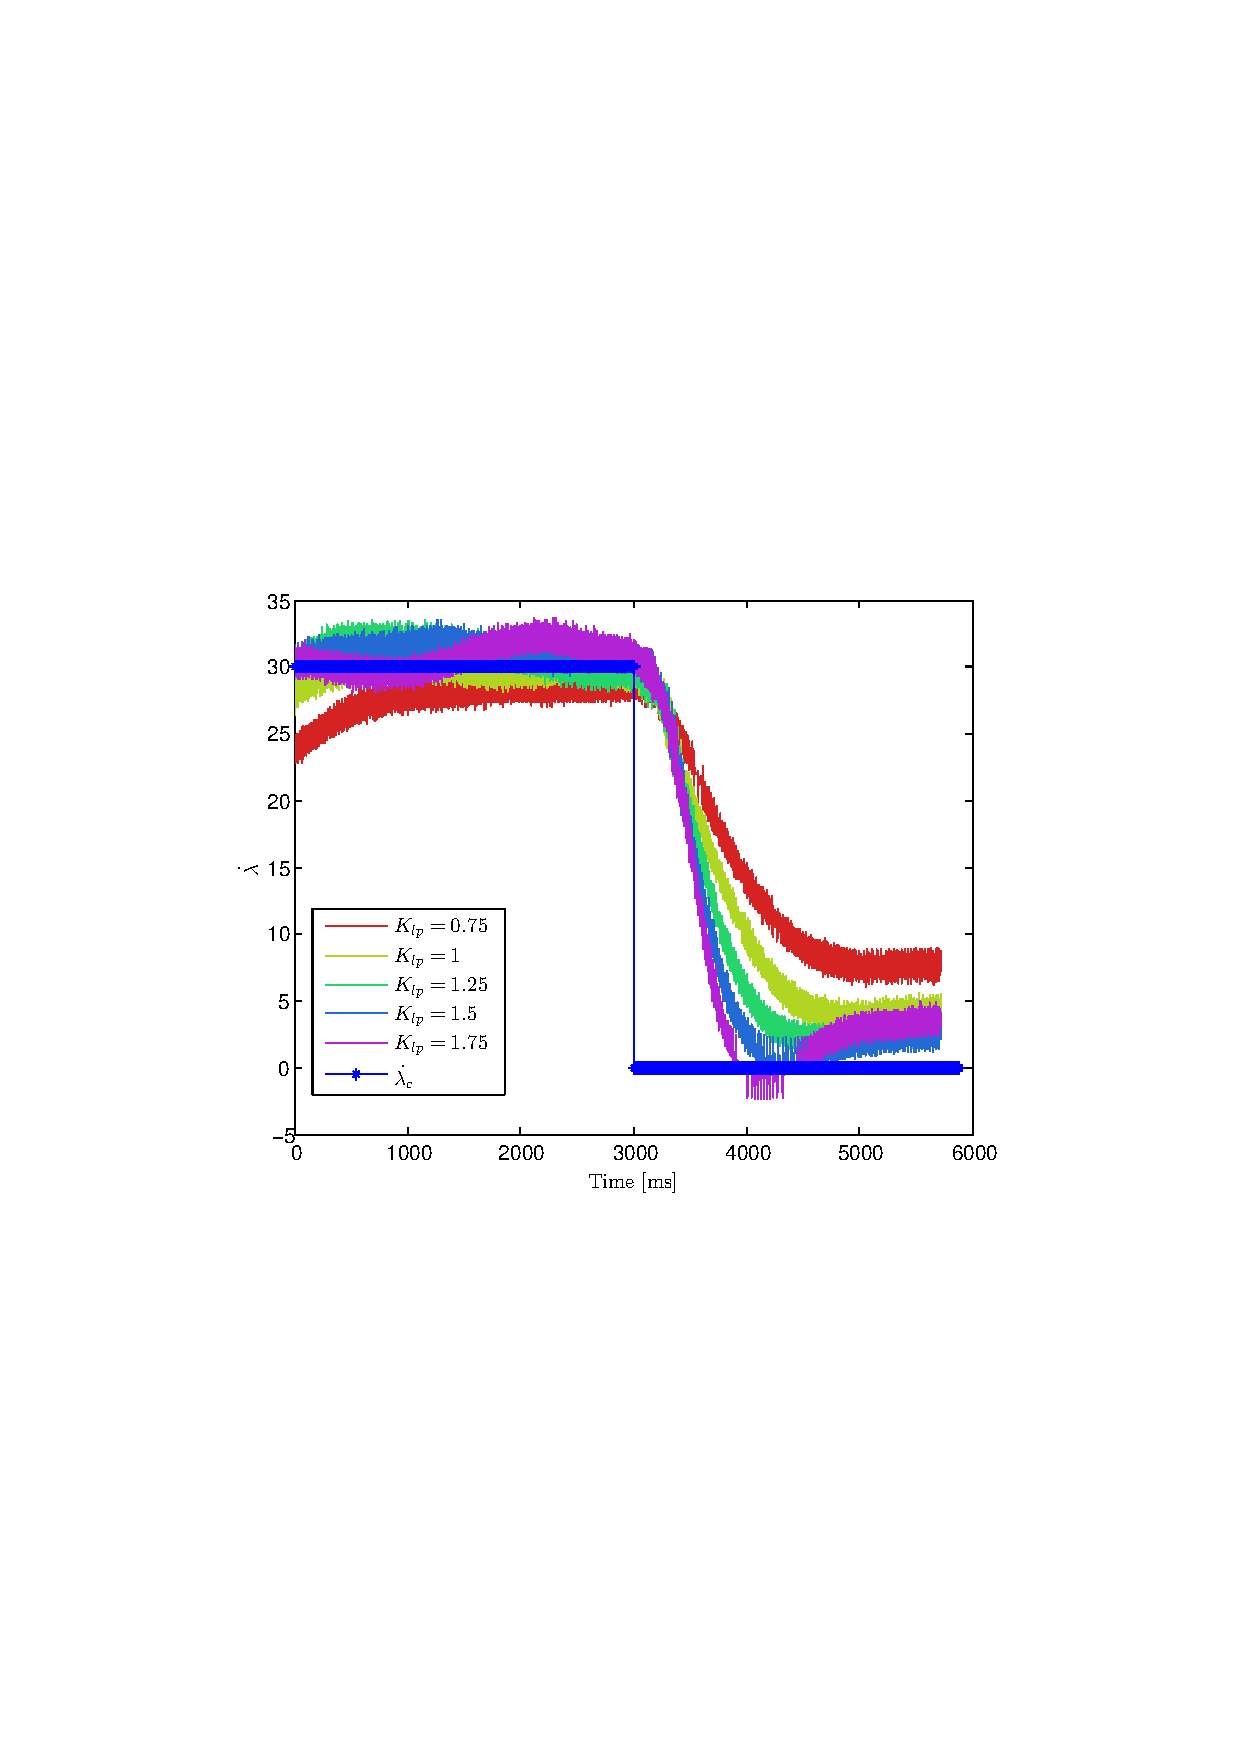
\includegraphics[width=1\textwidth,trim={4cm 9cm 4cm 9cm},clip]{figures/P2p2_Klp.pdf}
	\caption{Travel response with P control}
\label{fig:P2p2_K_lp}
\end{figure}
\clearpage
%%%%%%%%%%%%%%%%%%%%%%%%%%%%%%%%%%%%%%%%%%%%%%%%%%%%%%%%%%%%%%%%%%%%
\subsection{Part III - Multivariable control}



We don't need reference feed forward (P matrix) (F matrix???) when using integral effect. So we can use the same P matrix as in the previous problem. Sources on wikipendium and in Chen (Chapter 9 problem solutions 9.4).
\subsubsection{Problem 1}


Considering~\cref{eq:P1_lin_eq_of_motion} and a state vector and input of  

\begin{equation}\label{P3_state_vector_and_input}
    \mathbf{x}=
    \begin{bmatrix}
        \tilde{p}\\
        \td{p}\\
        \td{e}
    \end{bmatrix}
    \quad\text{and}\quad
    \mathbf{u}=
    \begin{bmatrix}
        \tilde{V_s}\\
        \tilde{V_d}
    \end{bmatrix}
\end{equation}

and a state-space formulation of the form
\begin{equation}\label{eq:P3_state_space_equation}
    \dot{\mathbf{x}}=\mathbf{Ax}+\mathbf{Bu}    
\end{equation}

the matrices $\mathbf{A}$ and $\mathbf{B}$ are given by 

\begin{subequations}\label{eq:P3_p1_A_B}
    \begin{align}
        \mathbf{A}=
            \begin{bmatrix}
                0&1&0\\
                0&0&0\\
                0&0&0
            \end{bmatrix}\label{eq:P3_p1_A} \\
        \mathbf{B}=
            \begin{bmatrix}
                0&0\\
                K_1&0\\
                0&K_2
            \end{bmatrix}\label{eq:P3_p1_B}.
    \end{align}
\end{subequations}

\subsubsection{Problem 2}

For this problem, the purpose was to track a reference

\begin{equation}\label{eq:P3_p2_reference}
    \mathbf{r}=
        \begin{bmatrix}
            \tilde{p_c}\\
            \dot{\tilde{e_c}}
        \end{bmatrix}
\end{equation}

Firstly, the controllability of the system is examined. Due to having three states, the controllability matrix is given by

\begin{equation}\label{eq:P3_p2_controllability_matrix}
    \mathcal{C}=
        \begin{bmatrix}
            \mathbf{B}&\mathbf{AB}&\mathbf{A^2B}
        \end{bmatrix}
\end{equation}

Using $K_1=0.9046$ and $K_2=0.1555$, the controllability matrix is given by

\begin{equation}
    \mathcal{C}=
        \begin{bmatrix}
            
        \end{bmatrix}
\end{equation}

Calculating the controllability matrix with 

\begin{figure}[!!ht!!!!!!!!tb!!]
	\centering
		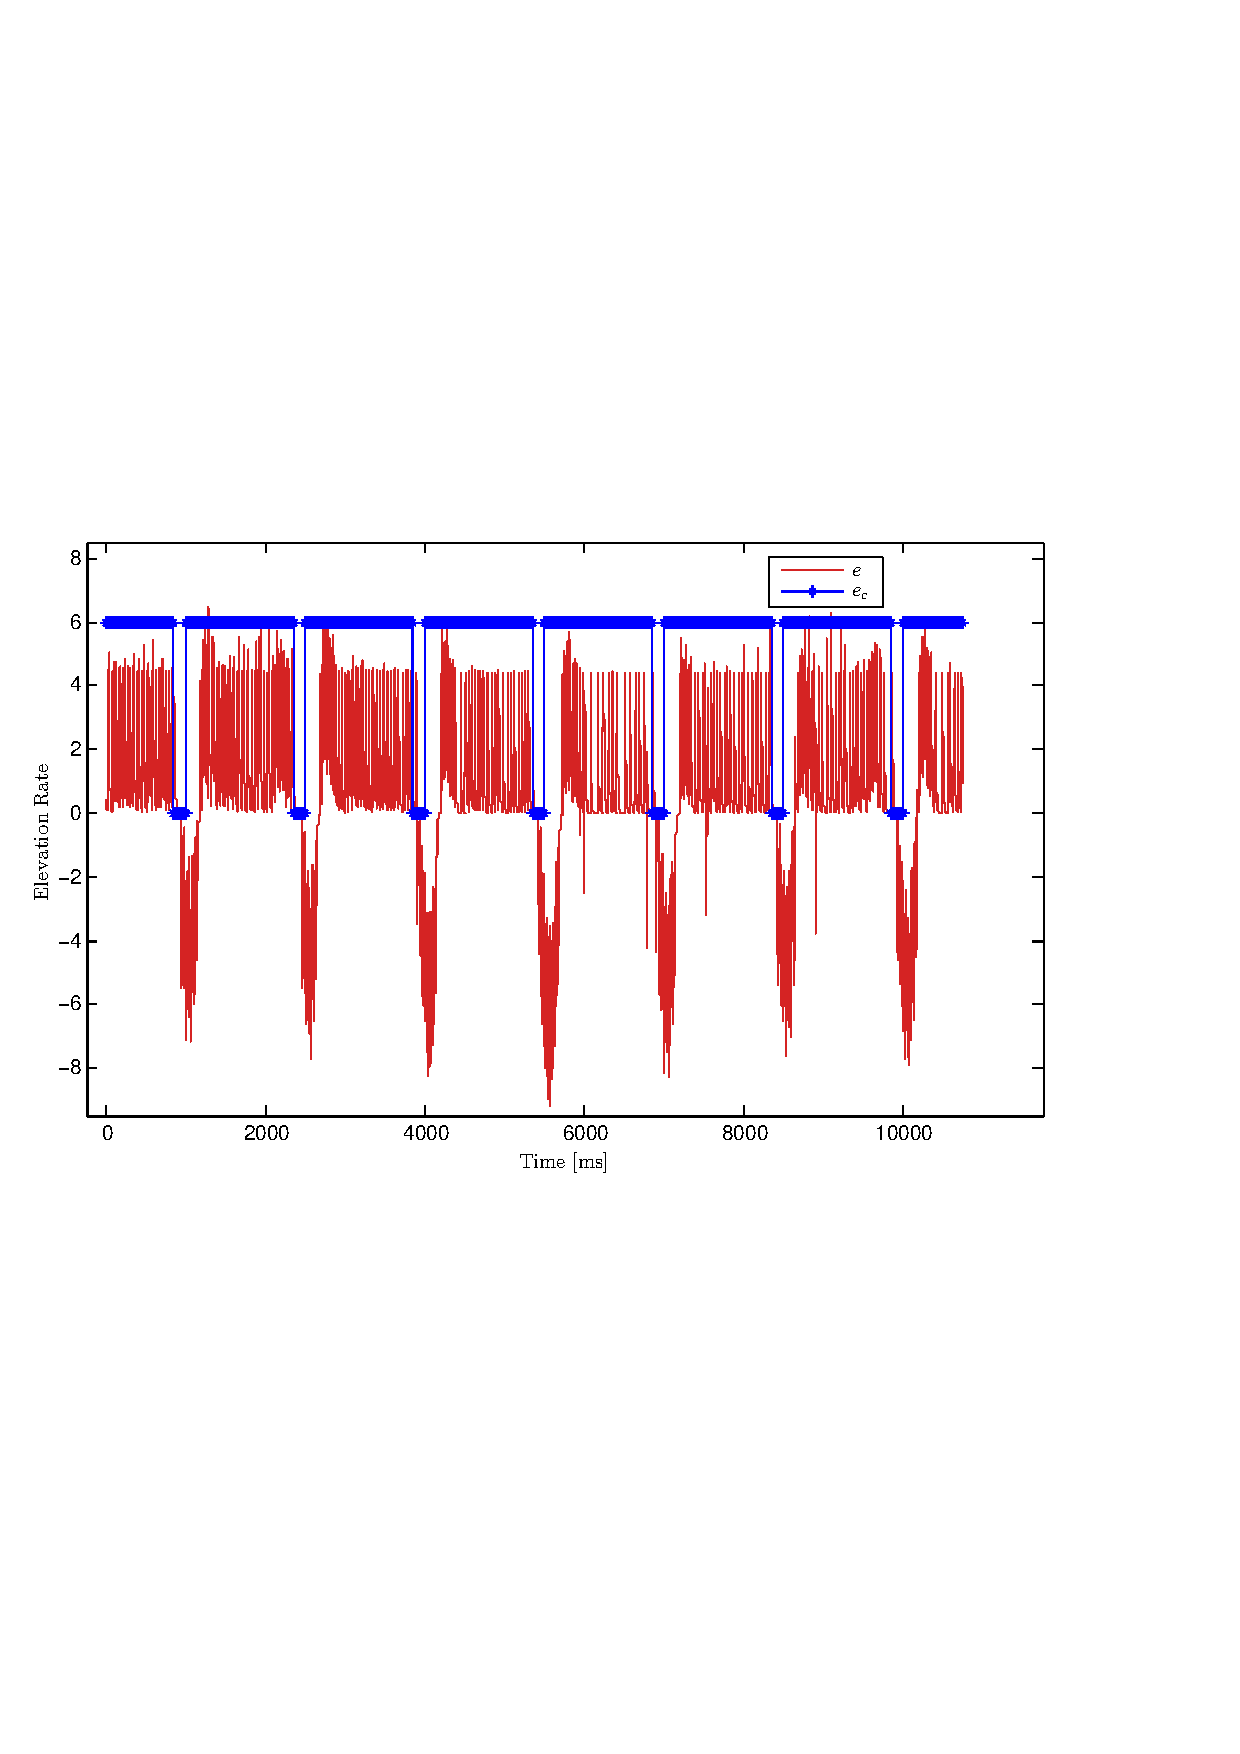
\includegraphics[width=1\textwidth,trim={4cm 9cm 4cm 9cm},clip]{figures/P3p2_e_dot.pdf}
	\caption{Travel response with P control}
\label{fig:P3p2_e_dot}
\end{figure}
\clearpage
\begin{figure}[!!ht!!!!!!!!tb!!]
	\centering
		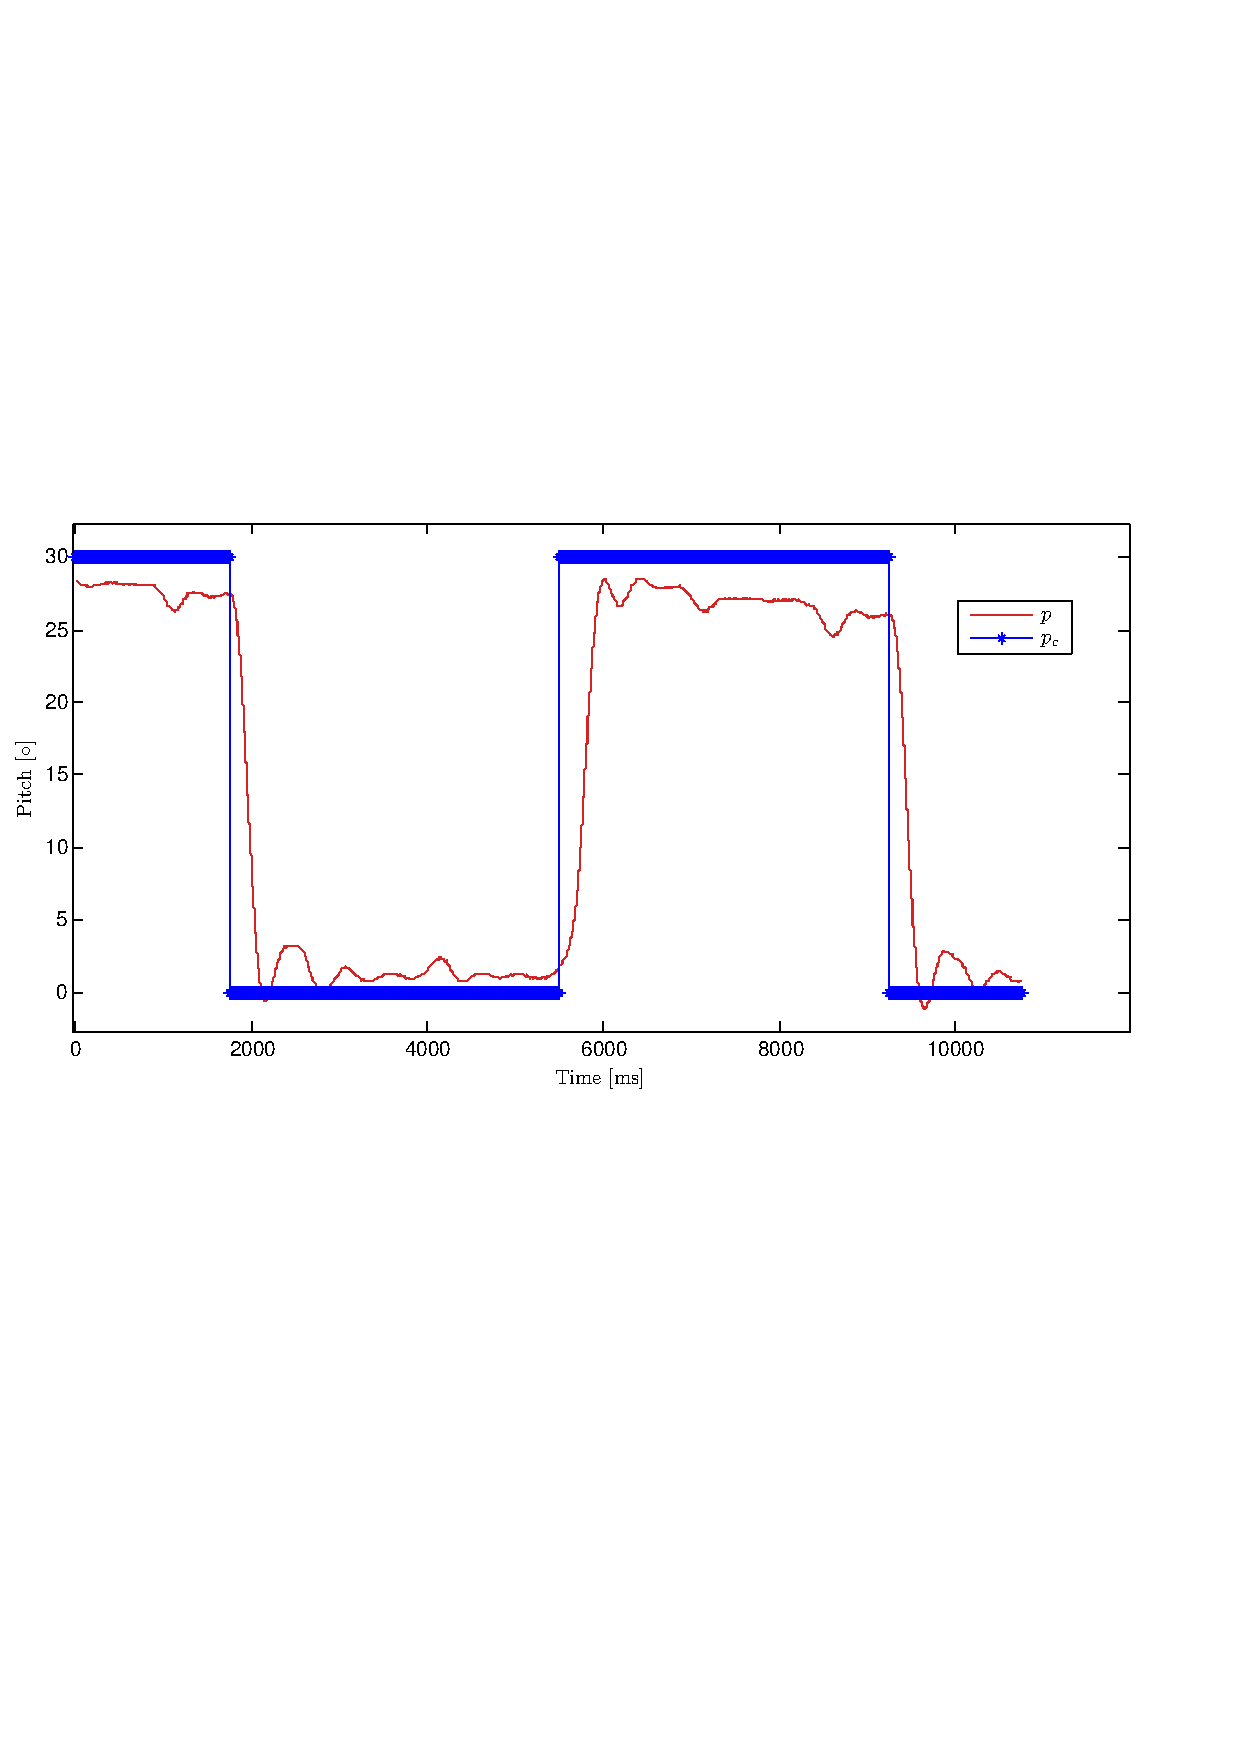
\includegraphics[width=1\textwidth,trim={4cm 9cm 4cm 9cm},clip]{figures/P3p2_p.pdf}
	\caption{Travel response with P control}
\label{fig:P3p2_p}
\end{figure}
\clearpage
%%%%%%%%%%%%%%%%%%%%%%%%%%%%%%%%%%%%%%%%%%%%%%%%%%%%%%%%%%%%%%%%%%%%
\subsection{Part IV - State estimation}









Answer all the parts of the exercise in an organized and clear manner. You should of course try to get good results in all the exercises, but if you have made a good effort without achieving great performance, a good discussion of possible reasons is just as good. Present your thinking and efforts and discuss possible reasons for good or bad results.

Include plots and/or tables of all relevant results, but make sure you don't overwhelm the reader with too many plots. Have a clear plan about what you want to communicate with a specific plot/figure, and use appropriate labels and comments. Keep in mind that the plots should be as ``readable'' as possible; that is, they should not be too hard to interpret and be reasonably self contained.

There are some important things to consider when exporting figures from MATLAB, most importantly which format you use. Always ever use JPEG for anything that is not a photography or similar. Any figure, like a plot or block diagram, must be stored as a JPEG\@. If you zoom in on \Cref{fig:constraint_jpg} you can see a lot of beauty close to any of the dark curves and lines, this is due to the lovely nature of JPEG\@. \Cref{fig:constraint_jpg} will look fantastic both on a screen and on paper.

The PNG format is slightly better for plots, but since it is a raster format (a grid of pixels), it looks ugly if you zoom in. It also looks ugly if you scale it, both on a screen and on paper. Try to avoid PNG if you can. \Cref{fig:constraint_png,fig:constraint_png_large} are both PNG figures; the latter being a larger figure scaled more than the former. Note both how choppy and ugly the blue curve is, and how the different sizes create inconsistent font sizes.

The simplest way to get a reasonably good looking plot is to save it as EPS in MATLAB\@. Do this by clicking ``File'' in the figure window, and the ``Save As\ldots''; choose ``EPS file (*.eps)'' in the ``Save as type:'' menu.\footnote{pdfLatex does not support EPS directly, but since we have loaded the \emph{epstodf} package, this is not a problem.} \Cref{fig:constraint_eps} shows a plot in EPS format. Since EPS is a vector format, the Figure can be scaled and still look good (but mind the font size!). If you zoom in you can see that the curve and the letters/numbers are smooth. A figure in vector format will usually look good both on a screen and on paper.

Note that the size of the actual figure window in MATLAB determines how large the exported figure is. Hence, if you enlarge the figure window before exporting, you will need to scale the figure by a larger factor in the report. This will lead to a tiny font in the figure. There are many better ways of exporting graphics from MATLAB, but they quickly become fairly involved. The above method of exporting to EPS will in most cases give nice figures.

You can write Latex in your MATLAB figures. The script used to create \Cref{fig:constraint_jpg,fig:constraint_eps} is included in \Cref{sec:plot_constraint_m}. Do not use a screen shot of a scope of figure in MATLAB in your report.


\begin{figure}[htb]
	\centering
		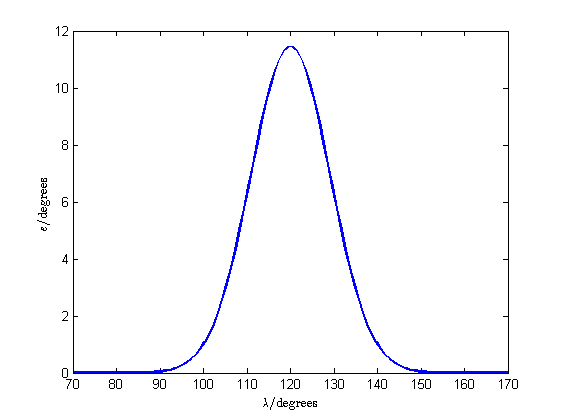
\includegraphics[width=0.8\textwidth]{figures/constraint_png.png}
	\caption{A plot in PNG format --- a bad idea.}
\label{fig:constraint_png}
\end{figure}

\begin{figure}[htb]
	\centering
		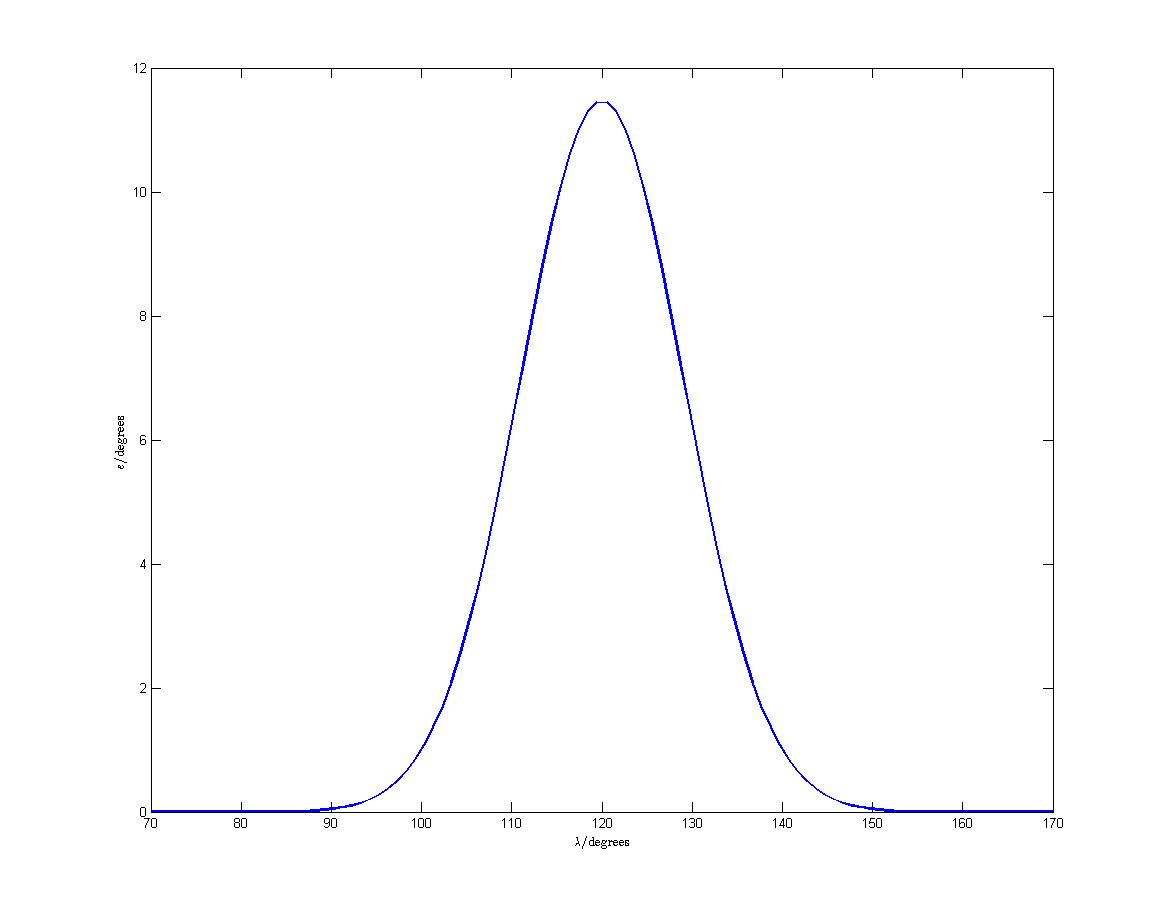
\includegraphics[width=0.8\textwidth]{figures/constraint_png_large.png}
	\caption{A plot in PNG format --- a bad idea. This figure is originally larger than the other PNG figure, but both are scaled to the same size.}
\label{fig:constraint_png_large}
\end{figure}

\begin{figure}[htb]
	\centering
		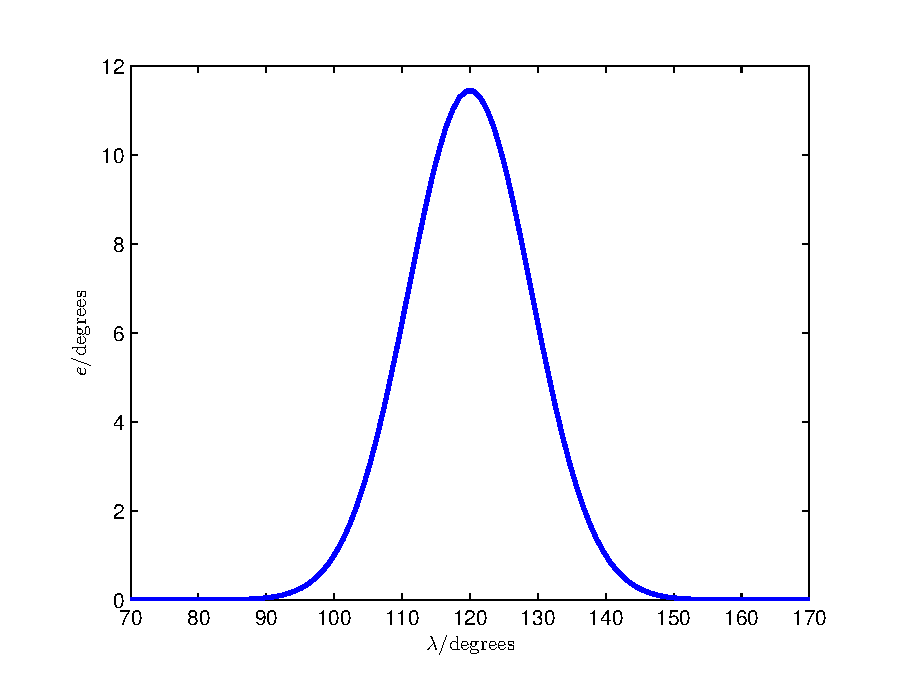
\includegraphics[width=0.8\textwidth]{figures/constraint_eps.eps}
	\caption{A plot in EPS format --- a much better idea.}
\label{fig:constraint_eps}
\end{figure}

Remember to reference all figures in the text. Figures have a number and should be referenced by that number (again, always use dynamic references). They also tend to float around, meaning they generally don't appear where you ask them to in the text. This is fine, do not try to force a figure (or a table) to appear in a particular place. As long a you refer to it, it's easy to find. No figure should be included without being referenced in the text.

If you look at the source code for including figures, you can see that the optional option \verb+[htb]+ has been used. This tells Latex where you wish the figure to appear, in prioritized order. \verb+h+ means ``Here'', t means ``Top of this page'', b means ``Bottom of this page'', and p (not used here) means ``on a Page with only floats (such as figures and tables)''. Note that your wish might not be granted, and this is because Latex actually optimizes the placement of figures. If you start forcing figures to be in specific places, it often leads to really strange layout somewhere else in the document. 

Generally, let Latex handle the documentation layout. This is one of the main reasons to choose Latex over software such as Microsoft Word.

\subsection{Results and Discussion}
All problems should have their own discussion of results. 

Remember: all plots and results need a description, explanation, and discussion.
